\begin{picture}(0,0)%
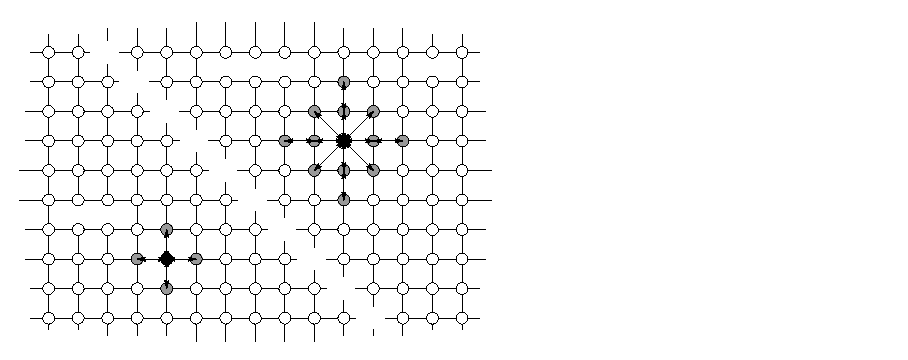
\epsfig{file=Skizzen/nnww3.ps}%
\end{picture}%
\setlength{\unitlength}{0.00087500in}%
%
\begingroup\makeatletter\ifx\SetFigFont\undefined
% extract first six characters in \fmtname
\def\x#1#2#3#4#5#6#7\relax{\def\x{#1#2#3#4#5#6}}%
\expandafter\x\fmtname xxxxxx\relax \def\y{splain}%
\ifx\x\y   % LaTeX or SliTeX?
\gdef\SetFigFont#1#2#3{%
  \ifnum #1<17\tiny\else \ifnum #1<20\small\else
  \ifnum #1<24\normalsize\else \ifnum #1<29\large\else
  \ifnum #1<34\Large\else \ifnum #1<41\LARGE\else
     \huge\fi\fi\fi\fi\fi\fi
  \csname #3\endcsname}%
\else
\gdef\SetFigFont#1#2#3{\begingroup
  \count@#1\relax \ifnum 25<\count@\count@25\fi
  \def\x{\endgroup\@setsize\SetFigFont{#2pt}}%
  \expandafter\x
    \csname \romannumeral\the\count@ pt\expandafter\endcsname
    \csname @\romannumeral\the\count@ pt\endcsname
  \csname #3\endcsname}%
\fi
\fi\endgroup
\begin{picture}(3624,2490)(214,-1828)
\put(586,-871){\makebox(0,0)[lb]{\smash{\SetFigFont{12}{14.4}{rm}{\tiny NN-WW}}}}
\put(1666,254){\makebox(0,0)[lb]{\smash{\SetFigFont{12}{14.4}{rm}{\tiny "ubern. N-WW}}}}
\put(3241,254){\makebox(0,0)[lb]{\smash{\SetFigFont{12}{14.4}{rm}{\tiny $d=2$}}}}
\end{picture}
